
\documentclass[a4paper,11pt]{article}
\usepackage[a4paper, margin=8em]{geometry}

% usa i pacchetti per la scrittura in italiano
\usepackage[french,italian]{babel}
\usepackage[T1]{fontenc}
\usepackage[utf8]{inputenc}
\frenchspacing 

% usa i pacchetti per la formattazione matematica
\usepackage{amsmath, amssymb, amsthm, amsfonts}

% usa altri pacchetti
\usepackage{gensymb}
\usepackage{hyperref}
\usepackage{standalone}

% imposta il titolo
\title{Appunti Elettronica Digitale}
\author{Luca Seggiani}
\date{2026}

% imposta lo stile
% usa helvetica
\usepackage[scaled]{helvet}
% usa palatino
\usepackage{palatino}
% usa un font monospazio guardabile
\usepackage{lmodern}

\renewcommand{\rmdefault}{ppl}
\renewcommand{\sfdefault}{phv}
\renewcommand{\ttdefault}{lmtt}

% disponi il titolo
\makeatletter
\renewcommand{\maketitle} {
	\begin{center} 
		\begin{minipage}[t]{.8\textwidth}
			\textsf{\huge\bfseries \@title} 
		\end{minipage}%
		\begin{minipage}[t]{.2\textwidth}
			\raggedleft \vspace{-1.65em}
			\textsf{\small \@author} \vfill
			\textsf{\small \@date}
		\end{minipage}
		\par
	\end{center}

	\thispagestyle{empty}
	\pagestyle{fancy}
}
\makeatother

% disponi teoremi
\usepackage{tcolorbox}
\newtcolorbox[auto counter, number within=section]{theorem}[2][]{%
	colback=blue!10, 
	colframe=blue!40!black, 
	sharp corners=northwest,
	fonttitle=\sffamily\bfseries, 
	title=~\thetcbcounter: #2, 
	#1
}

% disponi definizioni
\newtcolorbox[auto counter, number within=section]{definition}[2][]{%
	colback=red!10,
	colframe=red!40!black,
	sharp corners=northwest,
	fonttitle=\sffamily\bfseries,
	title=~\thetcbcounter: #2,
	#1
}

% U.D.M
\newcommand{\amp}{\ensuremath{\mathrm{A}}}
\newcommand{\volt}{\ensuremath{\mathrm{V}}}
\newcommand{\meter}{\ensuremath{\mathrm{m}}}
\newcommand{\second}{\ensuremath{\mathrm{s}}}
\newcommand{\farad}{\ensuremath{\mathrm{F}}}
\newcommand{\henry}{\ensuremath{\mathrm{H}}}
\newcommand{\siemens}{\ensuremath{\mathrm{S}}}

% circuiti
\usepackage{circuitikz}
\usetikzlibrary{babel}

% disegni
\usepackage{pgfplots}
\pgfplotsset{width=10cm,compat=1.9}

% disponi codice
\usepackage{listings}
\usepackage[table]{xcolor}

\definecolor{codegreen}{rgb}{0,0.6,0}
\definecolor{codegray}{rgb}{0.5,0.5,0.5}
\definecolor{codepurple}{rgb}{0.58,0,0.82}
\definecolor{backcolour}{rgb}{0.95,0.95,0.92}

\lstdefinestyle{codestyle}{
		backgroundcolor=\color{black!5}, 
		commentstyle=\color{codegreen},
		keywordstyle=\bfseries\color{magenta},
		numberstyle=\sffamily\tiny\color{black!60},
		stringstyle=\color{green!50!black},
		basicstyle=\ttfamily\footnotesize,
		breakatwhitespace=false,         
		breaklines=true,                 
		captionpos=b,                    
		keepspaces=true,                 
		numbers=left,                    
		numbersep=5pt,                  
		showspaces=false,                
		showstringspaces=false,
		showtabs=false,                  
		tabsize=2
}

\lstdefinestyle{shellstyle}{
		backgroundcolor=\color{black!5}, 
		basicstyle=\ttfamily\footnotesize\color{black}, 
		commentstyle=\color{black}, 
		keywordstyle=\color{black},
		numberstyle=\color{black!5},
		stringstyle=\color{black}, 
		showspaces=false,
		showstringspaces=false, 
		showtabs=false, 
		tabsize=2, 
		numbers=none, 
		breaklines=true
}

\lstdefinelanguage{javascript}{
	keywords={typeof, new, true, false, catch, function, return, null, catch, switch, var, if, in, while, do, else, case, break},
	keywordstyle=\color{blue}\bfseries,
	ndkeywords={class, export, boolean, throw, implements, import, this},
	ndkeywordstyle=\color{darkgray}\bfseries,
	identifierstyle=\color{black},
	sensitive=false,
	comment=[l]{//},
	morecomment=[s]{/*}{*/},
	commentstyle=\color{purple}\ttfamily,
	stringstyle=\color{red}\ttfamily,
	morestring=[b]',
	morestring=[b]"
}

% disponi sezioni
\usepackage{titlesec}

\titleformat{\section}
	{\sffamily\Large\bfseries} 
	{\thesection}{1em}{} 
\titleformat{\subsection}
	{\sffamily\large\bfseries}   
	{\thesubsection}{1em}{} 
\titleformat{\subsubsection}
	{\sffamily\normalsize\bfseries} 
	{\thesubsubsection}{1em}{}

% disponi alberi
\usepackage{forest}

\forestset{
	rectstyle/.style={
		for tree={rectangle,draw,font=\large\sffamily}
	},
	roundstyle/.style={
		for tree={circle,draw,font=\large}
	}
}

% disponi algoritmi
\usepackage{algorithm}
\usepackage{algorithmic}
\makeatletter
\renewcommand{\ALG@name}{Algoritmo}
\makeatother

% disponi numeri di pagina
\usepackage{fancyhdr}
\fancyhf{} 
\fancyfoot[L]{\sffamily{\thepage}}

\makeatletter
\fancyhead[L]{\raisebox{1ex}[0pt][0pt]{\sffamily{\@title \ \@date}}} 
\fancyhead[R]{\raisebox{1ex}[0pt][0pt]{\sffamily{\@author}}}
\makeatother

\begin{document}
% sezione (data)
\section{Lezione del 16-03-26}

% stili pagina
\thispagestyle{empty}
\pagestyle{fancy}

% testo
Abbiamo visto nella scrosa lezione come trattare i \textit{diodi} all'interno dei nostri circuiti. In particolare, avevamo dato una soglia $V_\gamma = 0.7 \, \mathrm{V}$ di "attivazione" del diodo.
\begin{itemize}
	\item Diciamo che quando questo si trova oltre la soglia, e quindi si comporta da conduttore, siamo nell'ipotesi di \textit{conduzione} del diodo;
	\item Diciamo che quando questo si trova al disotto la soglia, e quindi si comporta da aperto, siamo nell'ipotesi di \textit{interdizione} del diodo;
\end{itemize}
Risolvere circuiti contenenti diodi significa quindi fare ipotesi sulla conduzione o interdizione del diodo, e quindi verificare se tali ipotesi sono vere.

\subsection{Logica a diodi}
Iniziamo a vedere alcuni semplici circuiti in logica diodi, a partire della realizzazione di alcune \textbf{porte logiche}. Questo ci permetterà di mettere alla prova le tecniche per la risoluzione dei circuiti con diodi che abbiamo visto nelle ultime sezioni.

\subsubsection{Studio di una porta AND}
Vediamo come primo esempio di studio dei circuiti basati su diodi, l'analisi di un circuito che implementa una porta \textbf{AND}. Il circuito che prendiamo è il seguente:

\begin{center}
\begin{circuitikz}
	\node[anchor=east] at(0,0) {$A$};
	\node[anchor=east] at(0,-2) {$B$};
    \draw (2,0) to[diode, l=$D_A$] (0,0);
    \draw (2,-2) to[diode, l=$D_B$] (0,-2);
	\draw (2,-2) -- (2, 0) to [resistor, l=$R$] (2,2)
		-- (4,2) to[battery2, l=$V_{cc}$] (4,0);
	\draw (2,-1) -- (3,-1);
	\node[anchor=west] at(3,-1) {$V_u$};
	\node[ground] at(4,0) {};
\end{circuitikz}
\end{center}

Abbiamo quindi due diodi collegati ai capi $A$ e $B$, di cui assumiamo di poter variare il voltaggio $V_A$ e $V_B$ rispettivamente. $V_{cc}$ sarà la nostra sorgente di alimentazione, fissa a $5 \, \mathrm{V}$. Il valore di $R$ non è particolarmente significativo, ma come tutte le resistenze assumiamo che sia $R > 0$. $V_u$ sarà il valore di uscita che vogliamo modulare con $V_A$ e $V_B$.

Vediamo quindi tutte le possibili combinazioni di $A$ e $B$, assumendo di fissarli o a $0 \, \mathrm{V}$ o a $5 \, \mathrm{V}$.
Il risultato che ci aspettiamo di ottenere è quello dato dalla seguente tabella:
\begin{table}[h!]
	\center 
	\begin{tabular} { c | c || c }
		$V_A$ & $V_B$ & $V_u$ \\
		\hline
		$5 \, \mathrm{V}$ & $5 \, \mathrm{V}$ & $5 \, \mathrm{V}$ \\
		$0 \, \mathrm{V}$ & $5 \, \mathrm{V}$ & $0 \, \mathrm{V}$ \\
		$5 \, \mathrm{V}$ & $0 \, \mathrm{V}$ & $0 \, \mathrm{V}$ \\
		$0 \, \mathrm{V}$ & $0 \, \mathrm{V}$ & $0 \, \mathrm{V}$ \\
	\end{tabular}
\end{table}

\newpage

\begin{itemize}
\item $V_A = 5 \, \mathrm{V}, \quad V_B = 5 \, \mathrm{V}$ \\
La situazione si modellizza come segue:

\begin{center}
\begin{circuitikz}
	\draw (0, 0) to[battery2, l=$5 \, \mathrm{V}$] (-2, 0);
	\draw (0, -2) to[battery2, l=$5 \, \mathrm{V}$] (-2, -2);
    \draw (2,0) to[diode, l=$D_A$] (0,0);
    \draw (2,-2) to[diode, l=$D_B$] (0,-2);
	\draw (2,-2) -- (2, 0) to [resistor, l=$R$] (2,2)
		-- (4,2) to[battery2, l=$V_{cc}$] (4,0);
	\draw (2,-1) -- (3,-1);
	\node[anchor=west] at(3,-1) {$V_u$};
	\node[ground] at(4,0) {};
\end{circuitikz}
\end{center}

In questo caso vediamo che i diodi $D_A$ e $D_B$ hanno $+5 \, \mathrm{V}$ dal lato sinistro, e qualcosa di simile a $+ 5 \, \mathrm{V}$ dal lato destro (dalla sorgente $V_{cc}$). In verità potremmo prevedere di avere una caduta di potenziale su $R$, ma in ogni caso questo portera il voltaggio $V'$ a destra dei diodi a:
$$
V' = V_{cc} - I R < V_{cc}
$$
per qui in ogni caso i diodi si trovano a voltaggio 0, o addirittura in polarizzazione negativa. Questo significherà che possiamo considerarli come entrambi interdetti.

Se i diodi sono interdetti, allora il circuito non è neanche chiuso, e il voltaggio sul nodo $V_u$ sarà uguale al $V_{cc}$, cioé:
$$
V_u = 5 \, \mathrm{V}
$$

\par\smallskip
\textbf{\textsf{Verifica}}

La verifica in caso di diodi presi \textit{interdetti} si fa ponendo:
$$
V_{AK} < V_\gamma
$$
dove $V_{AK}$ è la differenza di potenziale fra anodo e catodo del diodo preso interdetto. In questo caso avremo che sia $D_A$ che $D_B$ sono stati presi interdetti, per cui:
$$
V_{D_A}, V_{D_B} < V_\gamma \approx 0.7 \, \mathrm{V}
$$
In questo caso, come abbiamo detto, i diodi sono a voltaggio 0 o in polarizzazione negativa, per cui:
$$
V_{D_A}, V_{D_B} < 0 \, \mathrm{V} \implies V_{D_A}, V_{D_B} < V_\gamma \approx 0.7 \, \mathrm{V}
$$
e l'ipotesi è verificata.

\newpage

\item $V_A = 0 \, \mathrm{V}, \quad V_B = 5 \, \mathrm{V}$ \\
La situazione si modellizza come segue:

\begin{center}
\begin{circuitikz}
	\node[ground] at(0,0) {};
	\draw (0, -2) to[battery2, l=$5 \, \mathrm{V}$] (-2, -2);
    \draw (2,0) to[diode, l=$D_A$] (0,0);
    \draw (2,-2) to[diode, l=$D_B$] (0,-2);
	\draw (2,-2) -- (2, 0) to [resistor, l=$R$] (2,2)
		-- (4,2) to[battery2, l=$V_{cc}$] (4,0);
	\draw (2,-1) -- (3,-1);
	\node[anchor=west] at(3,-1) {$V_u$};
	\node[ground] at(4,0) {};
\end{circuitikz}
\end{center}

In questo caso possiamo fare l'ipotesi che il diodo $D_B$, come nel caso precedente, sia in interdizione. Il diodo $D_A$, invece, si troverà a chiudere un circuito diretto fra $V_{cc}$ e ground, per cui potremmo prenderlo come in conduzione.

In tal caso, sarà immediato notare (preso il modello a diodo ideale) che a sinistra e a destra di $D_A$ siamo collegati direttamente al ground, per cui il voltaggio al nodo $V_u$ è nullo, cioè:
$$
V_u = 0 \, \mathrm{V}
$$

\par\smallskip
\textbf{\textsf{Verifica}}

La verifica in caso di diodi presi \textit{conduttori} si fa ponendo:
$$
I_d > 0
$$
dove $I_d$ è la corrente sul diodo. Nel nostro circuito, abbiamo che la corrente sul diodo in conduzione $D_A$ è:
$$
I_{D_A} = \frac{V_{cc}}{R} > 0
$$
in quanto $V_{cc} > 0$ e $R$, come tutte le resistenze, è $R > 0$.

Per quanto riguarda $D_B$, invece, lo abbiamo preso in interdizione e quindi applichiamo la formula di verifica del caso precedente:
$$
V_{AK} = V_{D_B} = -5 \, \mathrm{V} < V_\gamma
$$

\item $V_A = 5 \, \mathrm{V}, \quad V_B = 0 \, \mathrm{V}$ \\
La situazione si modellizza come segue:
\begin{center}
\begin{circuitikz}
	\draw (0, 0) to[battery2, l=$5 \, \mathrm{V}$] (-2, 0);
	\node[ground] at(0,-2) {};
    \draw (2,0) to[diode, l=$D_A$] (0,0);
    \draw (2,-2) to[diode, l=$D_B$] (0,-2);
	\draw (2,-2) -- (2, 0) to [resistor, l=$R$] (2,2)
		-- (4,2) to[battery2, l=$V_{cc}$] (4,0);
	\draw (2,-1) -- (3,-1);
	\node[anchor=west] at(3,-1) {$V_u$};
	\node[ground] at(4,0) {};
\end{circuitikz}
\end{center}

Qui vale l'ipotesi opposta alla precedente: $D_A$ sarà in interdizione mentre $D_B$ sarà in conduzione (in quanto chiude un circuito diretto fra $V_{cc}$ e ground).

Come prima, vale che a sinistra e a destra di $D_B$ siamo collegati direttamente al ground, per cui il voltaggio al nodo $V_u$ è nullo, cioè:
$$
V_u = 0 \, \mathrm{V}
$$

\par\smallskip
\textbf{\textsf{Verifica}}

La verifica si fa in maniera analoga al caso precedente. Nel nostro circuito, abbiamo che la corrente sul diodo in conduzione $D_B$ è:
$$
I_{D_B} = \frac{V_{cc}}{R} > 0
$$
che è subito dimostrato, mentre per quanto riguarda $D_A$ lo abbiamo preso in interdizione e quindi applichiamo la formula di verifica del caso precedente:
$$
V_{AK} = V_{D_B} = -5 \, \mathrm{V} < V_\gamma
$$

\item $V_A = 0 \, \mathrm{V}, \quad V_B = 0 \, \mathrm{V}$ \\ 
La situazione si modellizza come segue:
\begin{center}
\begin{circuitikz}
	\node[ground] at(0,0) {};
	\node[ground] at(0,-2) {};
    \draw (2,0) to[diode, l=$D_A$] (0,0);
    \draw (2,-2) to[diode, l=$D_B$] (0,-2);
	\draw (2,-2) -- (2, 0) to [resistor, l=$R$] (2,2)
		-- (4,2) to[battery2, l=$V_{cc}$] (4,0);
	\draw (2,-1) -- (3,-1);
	\node[anchor=west] at(3,-1) {$V_u$};
	\node[ground] at(4,0) {};
\end{circuitikz}
\end{center}

In questo caso ci si aspetta che entrambi i diodi $D_A$ e $D_B$ siano in conduzione, in quanto fanno parte di un circuito diretto da $V_{cc}$ al ground.

Abbiamo quindi lo stesso risultato di prima:
$$
V_u = 0 \, \mathrm{V}
$$
dato dal fatto che $V_u$ si trova sullo stesso polo di $D_A$ e $D_B$ (presi come ideali), collegato al ground.

\par\smallskip
\textbf{\textsf{Verifica}}

La verifica si fa verificando l'ipotesi di conduzione, e quindi prendendo:
$$
I_d > 0, \quad I_{D_A}, I_{D_B} > 0
$$
che è verificata considerando che sui due rami passa la corrente:
$$
I_R = \frac{V_{cc}}{R} > 0
$$

\end{itemize}

Adesso, verificati tutti i casi, assegnamo dei valori logici ai voltaggi $V_A$, $V_B$ e $V_u$. Diciamo ad esempio che:
\begin{itemize}
	\item $0 \, \mathrm{V}$ corrisponde al valore logico \textit{falso};
	\item $5 \, \mathrm{V}$ corrisponde al valore logico \textit{vero}.
\end{itemize}

Applicando tale associazione alla tabella dei voltaggi riportata sopra otteniamo:
\begin{table}[h!]
	\center 
	\begin{tabular} { c | c || c }
		$A$ & $B$ & $u$ \\
		\hline
		$1$ & $1$ & $1$ \\
		$0$ & $1$ & $0$ \\
		$1$ & $0$ & $0$ \\
		$0$ & $0$ & $0$ \\
	\end{tabular}
\end{table}

Vediamo quindi che il circuito implementa la tavola di verità dell'operazione di congiunzione logica, e quindi l'AND logico. Notiamo che questo è il modo in cui implementiamo tutte le \textit{porte logiche}:
\begin{itemize}
	\item Nel dominio \textit{analogico}, creiamo circuiti che manipolano voltaggi e correnti in modo da ottenere i risultati desiderati;
	\item Solo dopo, assegnamo a determinati range di corrente o voltaggio dei valori logici, in modo da implementare operazioni nel cosiddetto dominio \textit{logico}.

		In tal caso, visto che i valori analogici sono \textit{reali} $\in \mathbb{R}$, e non valori discreti, dobbiamo definire dei \textit{range} di validità dei valori falsi o veri rappresentati dal voltaggio. Fra i due ci sarà una zona di indeterminazione, che vorremo evitare, e tollereremo solo in particolari situazioni transienti.
\begin{center}
	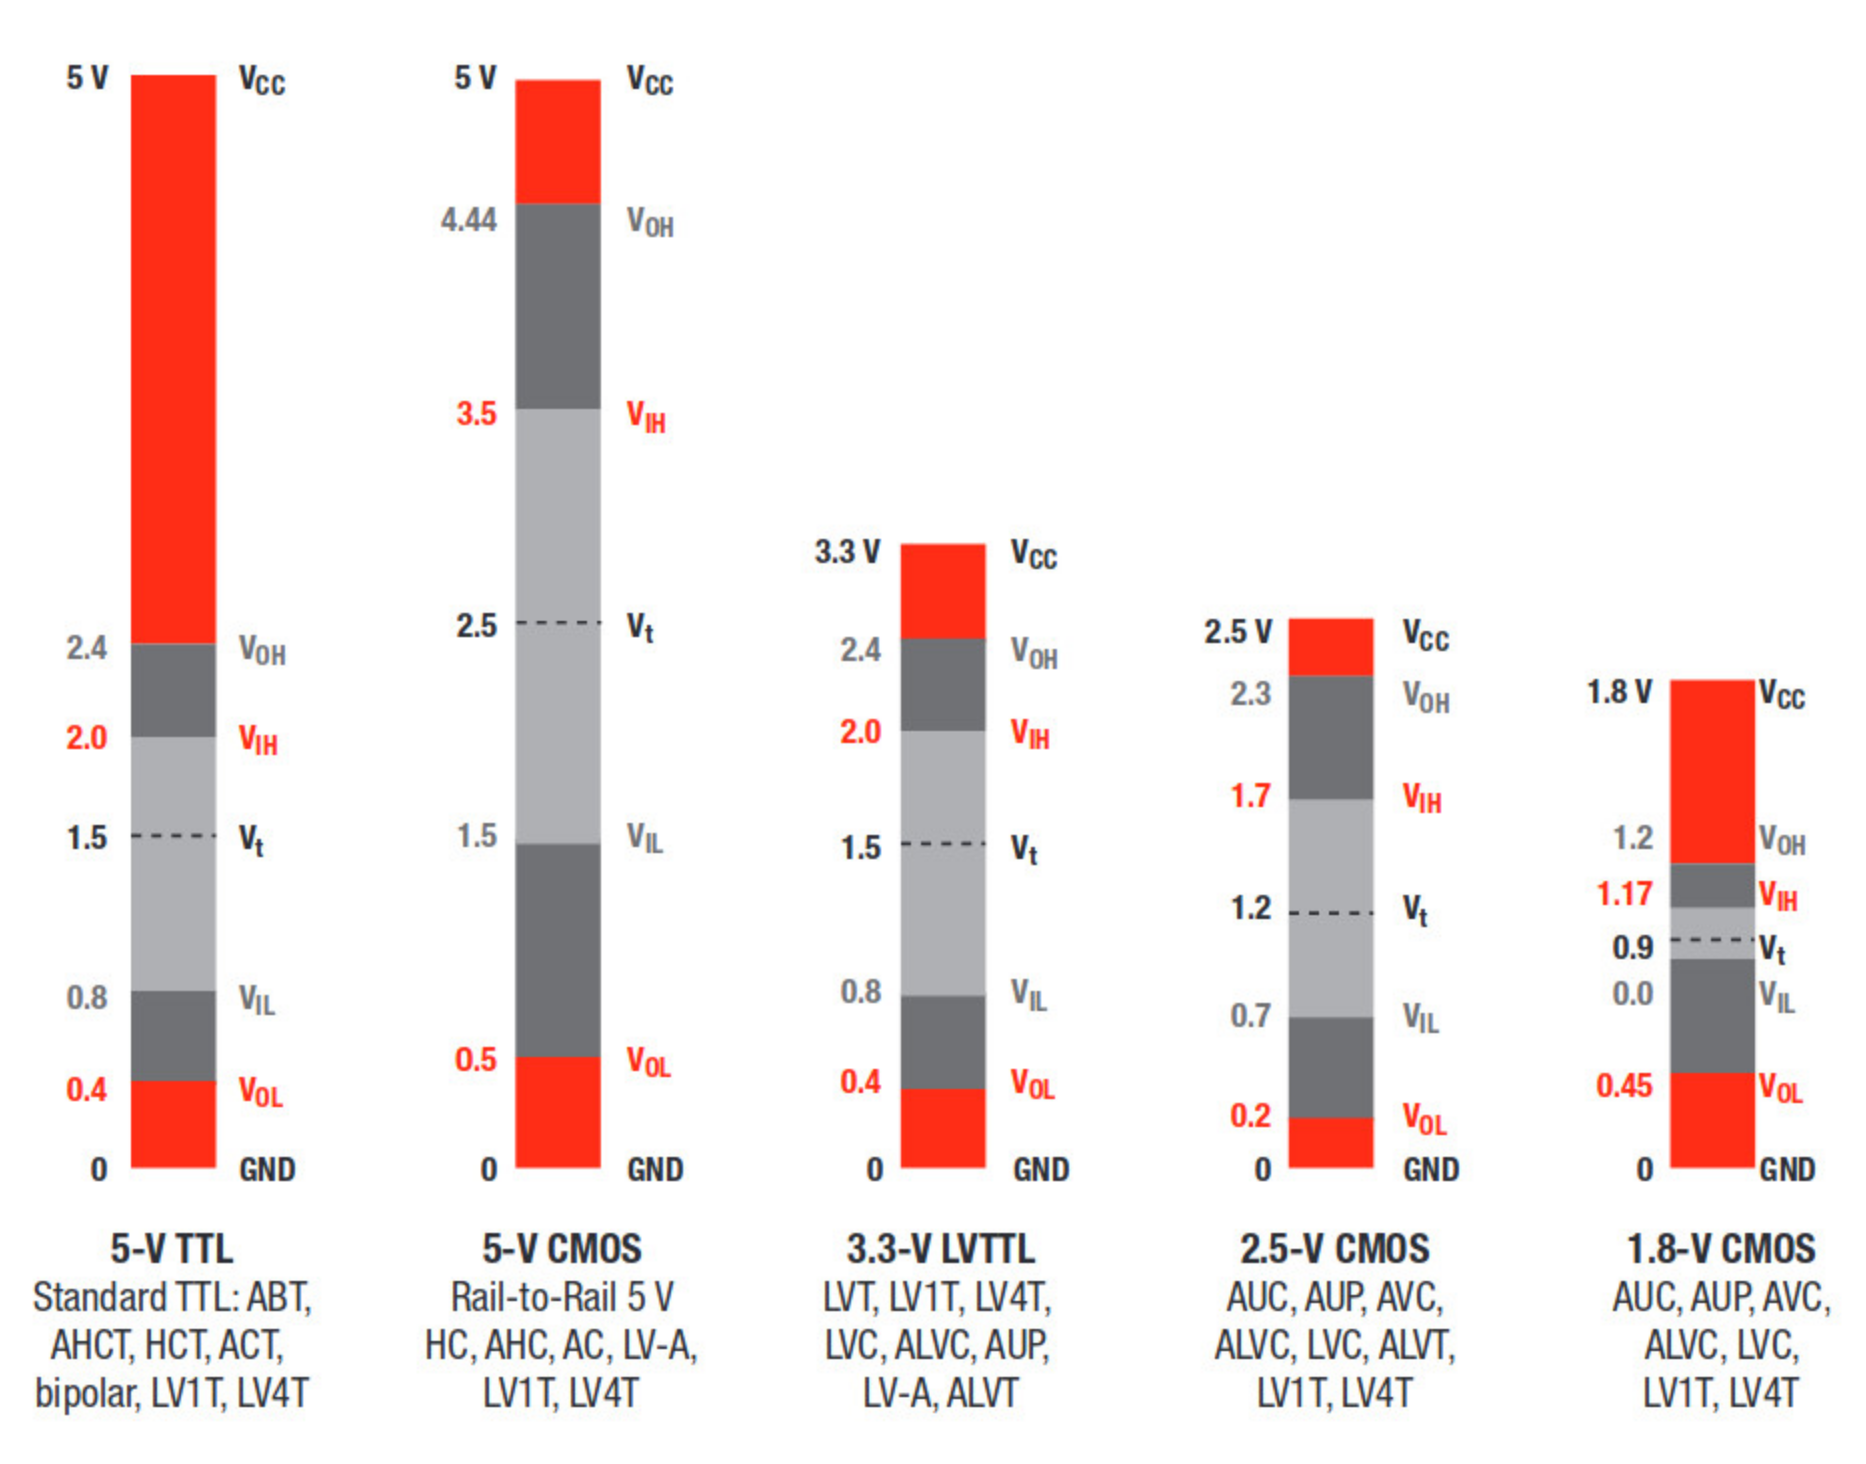
\includegraphics[scale=0.2]{../figures/logic_level.png}
\end{center}

		In particolare, noi abbiamo scelto $5 \, \mathrm{V}$ come riferimento per il \textit{vero} logico. Questo è il valore tipico della logica a diodi o a transistor (\textbf{TTL}, \textit{Transistor-Transistor Logic}). Le moderne applicazioni \textbf{CMOS} (\textit{Complementary Metal-Oxide-Semiconductor} usano invece valori come $3.3 \, \mathrm{V}$, $2.5 \, \mathrm{V}$ o addirittura $1.8 \, \mathrm{V}$.
\end{itemize}

\subsubsection{Studio di una porta OR}
Come abbiamo visto una porta \textit{AND}, vediamo a scopo di esempio anche una porta \textbf{OR}. Il circuito che prendiamo è il seguente:

\begin{center}
\begin{circuitikz}
	\node[anchor=east] at(0,0) {$A$};
	\node[anchor=east] at(0,-2) {$B$};
    \draw (0,0) to[diode, l=$D_A$] (2,0);
    \draw (0,-2) to[diode, l=$D_B$] (2,-2);
	\draw (2,0) -- (2, -2) to [resistor, l=$R$] (2,-4);
	\draw (2,-1) -- (3,-1);
	\node[anchor=west] at(3,-1) {$V_u$};
	\node[ground] at(2,-4) {};
\end{circuitikz}
\end{center}

In questo caso abbiamo sempre i morsetti $A$ e $B$, e i relativi diodi $D_A$ e $D_B$, che faranno da ingressi della porta, e il morsetto $V_u$, che farà da uscita.
Notiamo invece la particolarità di non avere un generatore di tensione $V_{cc}$: la porta è quindi completamente \textit{passiva}.

Come prima, quindi, vediamo tutte le possibili combinazioni di $A$ e $B$, assumendo di fissarli o a $0 \, \mathrm{V}$ o a $5 \, \mathrm{V}$.
Il risultato che ci aspettiamo di ottenere è quello dato dalla seguente tabella:
\begin{table}[h!]
	\center 
	\begin{tabular} { c | c || c }
		$V_A$ & $V_B$ & $V_u$ \\
		\hline
		$5 \, \mathrm{V}$ & $5 \, \mathrm{V}$ & $5 \, \mathrm{V}$ \\
		$0 \, \mathrm{V}$ & $5 \, \mathrm{V}$ & $5 \, \mathrm{V}$ \\
		$5 \, \mathrm{V}$ & $0 \, \mathrm{V}$ & $5 \, \mathrm{V}$ \\
		$0 \, \mathrm{V}$ & $0 \, \mathrm{V}$ & $0 \, \mathrm{V}$ \\
	\end{tabular}
\end{table}

\newpage

\begin{itemize}
\item $V_A = 5 \, \mathrm{V}, \quad V_B = 5 \, \mathrm{V}$ \\
La situazione si modellizza come segue:
\begin{center}
\begin{circuitikz}
	\draw (0, 0) to[battery2, l=$5 \, \mathrm{V}$] (-2, 0);
	\draw (0, -2) to[battery2, l=$5 \, \mathrm{V}$] (-2, -2);
    \draw (0,0) to[diode, l=$D_A$] (2,0);
    \draw (0,-2) to[diode, l=$D_B$] (2,-2);
	\draw (2,0) -- (2, -2) to [resistor, l=$R$] (2,-4);
	\draw (2,-1) -- (3,-1);
	\node[anchor=west] at(3,-1) {$V_u$};
	\node[ground] at(2,-4) {};
\end{circuitikz}
\end{center}

In questo caso entrambi i diodi $D_A$ e $D_B$ saranno in conduzione, in quanto chiuderanno un circuito con il ground attraverso $R$.

Avremo quindi che $V_u$ è parte del polo formato da $D_A$ e $D_B$, e la sua tensione sarà di conseguenza uguale a $V_{D_A}$ e $V_{D_B}$:
$$
V_u = 5 \, \mathrm{V}
$$

\par\smallskip
\textbf{\textsf{Verifica}}

Per ipotesi di conduzione verifichiamo che la corrente sia non negativa, per cui:
$$
I_d > 0, \quad I_{D_A} = I_{D_B} = \frac{5 \, \mathrm{V}}{R} > 0
$$

\item $V_A = 0 \, \mathrm{V}, \quad V_B = 5 \, \mathrm{V}$ \\
La situazione si modellizza come segue:
\begin{center}
\begin{circuitikz}
	\node[ground] at(0,0) {};
	\draw (0, -2) to[battery2, l=$5 \, \mathrm{V}$] (-2, -2);
    \draw (0,0) to[diode, l=$D_A$] (2,0);
    \draw (0,-2) to[diode, l=$D_B$] (2,-2);
	\draw (2,0) -- (2, -2) to [resistor, l=$R$] (2,-4);
	\draw (2,-1) -- (3,-1);
	\node[anchor=west] at(3,-1) {$V_u$};
	\node[ground] at(2,-4) {};
\end{circuitikz}
\end{center}

In questo caso $D_A$ sarà in interdizione, portato a $5 \, \mathrm{V}$ sul catodo dal diodo $D_B$ (che di per sè sarà in conduzione). Vediamo qui l'utilità del diodo ad impedire che la corrente passi all'opposto della direzione desiderata (cioè imporre che non passi dal diodo $D_B$ a $5 \, \mathrm{V}$ al ground a sinistra di $D_A$). 

La situazione in uscita non cambia in quanto il polo su $V_u$ resta pilotato da voltaggio applicato a $D_B$, e quindi:
$$
V_u = 5 \, \mathrm{V}
$$

\par\smallskip
\textbf{\textsf{Verifica}}

Abbiamo fatto l'ipotesi di interdizione su $D_A$, per cui applichiamo la verifica del voltaggio:
$$
V_{D_A} < 0 \implies V_{D_A} < V_\gamma \approx 0.7 \, \mathrm{V}
$$
in quanto abbiamo detto $D_A$ è in polarizzazione negativa.

Per quanto riguarda $D_B$, invece, vogliamo verificare $I_d > 0$:
$$
I_d = I_{D_B} > 0 = \frac{5 \, \mathrm{V}}{R} > 0
$$

\item $V_A = 5 \, \mathrm{V}, \quad V_B = 0 \, \mathrm{V}$ \\
La situazione si modellizza come segue:
\begin{center}
\begin{circuitikz}
	\draw (0, 0) to[battery2, l=$5 \, \mathrm{V}$] (-2, 0);
	\node[ground] at(0,-2) {};
    \draw (0,0) to[diode, l=$D_A$] (2,0);
    \draw (0,-2) to[diode, l=$D_B$] (2,-2);
	\draw (2,0) -- (2, -2) to [resistor, l=$R$] (2,-4);
	\draw (2,-1) -- (3,-1);
	\node[anchor=west] at(3,-1) {$V_u$};
	\node[ground] at(2,-4) {};
\end{circuitikz}
\end{center}

In questo caso $D_B$ sarà in interdizione, portato a $5 \, \mathrm{V}$ sul catodo dal diodo $D_A$ (che di per sè sarà in conduzione), in una situazione completamente opposta alla precedente. 

La situazione in uscita ancora una volta non cambia in quanto il polo su $V_u$ resta pilotato da voltaggio applicato a $D_A$, e quindi:
$$
V_u = 5 \, \mathrm{V}
$$

\par\smallskip
\textbf{\textsf{Verifica}}

Abbiamo fatto l'ipotesi di interdizione su $D_B$, per cui applichiamo la verifica del voltaggio:
$$
V_{D_B} < 0 \implies V_{D_B} < V_\gamma \approx 0.7 \, \mathrm{V}
$$
in quanto abbiamo detto $D_B$ è in polarizzazione negativa.

Per quanto riguarda $D_A$, invece, vogliamo verificare $I_d > 0$:
$$
I_d = I_{D_A} > 0 = \frac{5 \, \mathrm{V}}{R} > 0
$$

\item $V_A = 0 \, \mathrm{V}, \quad V_B = 0 \, \mathrm{V}$ \\ 
La situazione si modellizza come segue:
\begin{center}
\begin{circuitikz}
	\node[ground] at(0,0) {};
	\node[ground] at(0,-2) {};
    \draw (0,0) to[diode, l=$D_A$] (2,0);
    \draw (0,-2) to[diode, l=$D_B$] (2,-2);
	\draw (2,0) -- (2, -2) to [resistor, l=$R$] (2,-4);
	\draw (2,-1) -- (3,-1);
	\node[anchor=west] at(3,-1) {$V_u$};
	\node[ground] at(2,-4) {};
\end{circuitikz}
\end{center}

In questo caso la rete è triviale in quanto non presenta nemmeno un generatore di tensione. Tutto è connesso al ground, e quindi tutto è a $0 \, \mathrm{V}$. Possiamo assumere che diodi siano in interdizione, in quanto il voltaggio che hanno ad entrambi i lati è nullo.

\par\smallskip
\textbf{\textsf{Verifica}}

Per i diodi $D_A$ e $D_B$ in interdizione, e tutta la rete a $0 \, \mathrm{V}$, la verifica è banale:
$$
V_{D_A} = V_{D_B} = 0 < V_\gamma \approx 0.7 \, \mathrm{V} 
$$

\end{itemize}

Risulta immediato, applicando lo stesso schema di valori logici di prima, che abbiamo ricavato la tabella:
\begin{table}[H]
	\center 
	\begin{tabular} { c | c || c }
		$A$ & $B$ & $u$ \\
		\hline
		$1$ & $1$ & $1$ \\
		$0$ & $1$ & $1$ \\
		$1$ & $0$ & $1$ \\
		$0$ & $0$ & $0$ \\
	\end{tabular}
\end{table}
cioè la tabella di verità di una porta OR, che è ciò che ci eravamo prefissati di fare.

\subsubsection{Pregi e difetti della logica a diodi}
Abbiamo quindi visto alcuni semplici circuiti digitali in logica a diodi. Abbiamo che questi sono molto semplici (sia da capire che da realizzare), in quanto coinvolgono solo componenti semplici (diodi, resistenze, ecc...). Nonostante ciò, abbiamo che la logica a diodi ha delle problematiche:
\begin{itemize}
	\item La corrente in entrata alle porte $I \neq 0$ può essere diversa da 0: questo è problematico in quanto ci piacerebbe avere una "interfaccia" comune ai nostri componenti (magari codificando i valori logici solo attraverso la tensione, e non attraverso la corrente);
	\item Visto che i circuiti reali non sono ideali, si ha un certo grado di \textit{degradazione} del segnale. Ciò significa che la corrente e le tensioni in uscita dalle porte non sono pari al $V_{cc}$ di $5 \, \mathrm{V}$, ma leggermente minori. Il risultato sarà che collegando diverse porte in \textit{cascata} si avrà una degradazione del segnale che eventualmente renderà i nostri circuiti inutilizzabili. 

		Questo problamea è eliminato ad esempio dalla logica CMOS), che invece compie un operazione di \textit{rigenerazione} del segnale sulle porte;
	\item Infine, con la sola logica a diodi, non si ha a disposizione nessun tipo di \textit{inverter} (porta logica NOT). Vediamo che questo non ci permette di realizzare tutta la logica booleana, e quindi rende la logica a diodi effettivamente per i calcolatori.

		Una soluzione sarà data dalla logica a transistor, attraverso la quale è semplice realizzare ad esempio la porta \textbf{NAND}, che dagli anni '50 è stata alla base della logica digitale (ricordiamo che una NAND può formare una NOT connettendo gli ingressi fra di loro);
\end{itemize}

Inoltre, ci sono diverse caratteristiche da tenere a mente quando si progettano circuiti (in qualsiasi tipo di logica). Ad esempio:
\begin{itemize}
	\item Il livello di \textit{porte in cascata} è da considerare sia che si abbiano i problemi di degradazione della logica a diodi che no, in quanto si hanno tradeoff in termini di tempo di transizione, o spazio occupato delle porte. Dai corsi di reti logiche, ricordiamo che esistono svariate tecniche di decomposizione dei circuiti logici, ricavate dalla logica booleana, che possono permetterci di realizzare lo stesso circuito logico usando più o meno porte;
	\item Anche i tradeoff legati alla \textit{potenza} consumata dai circuiti in proporzione alla loro velocità sono da considerare: in generale, vorremo velocità più grandi possibili per diminuire i tempi di risposta, ma questo non viene se non compromettendo sulla potenza usata. Ad esempio, nella realizzazione di memorie digitali, sfruttiamo capacità. Per caricare più velocemente una capacità, è intuitivo che bisogna aumentare la corrente in entrata $I$. Ora, se la potenza è data da:
		$$
		P = I^2 R
		$$
allora sarà semplice notare che maggiori velocità di carica corrispondono in linea di massima a maggiore potenza usata;
\item Infine, consideriamo l'impatto che la struttura delle porte può avere sulla \textit{superficie} del circuito. In generale i circuiti si pagano al $\mathrm{mm}^2$, per cui realizzare lo stesso circuito su una \textit{footprint} minore può portare a risparmi energetici. Inoltre, la distanza fra i componenti, il loro numero, ecc... possono ancora influire sui tempi di risposta e di transizione, particolarmente importanti nei circuiti digitali. Anche in questo caso ci aiuta passare dalla logica a diodi o transistor ad altri tipi di logica come CMOS.
\end{itemize}

\subsection{Circuiti rettificatori}
Un applicazione tipica dei diodi è quella della \textbf{rettificazione} della tensione. La rettificazione è un operazione che porta una corrente alternata in una corrente continua, o comunque porta una tensione che oscilla attorno ad uno $0$ di potenziale a stare tutta sopra tale 0.

Circuiti di questo tipo sono utili ad esempio per ottenere generatori di tensione stabili dalla comune alimentazione casalinga ($311 \, \mathrm{V}$ di picco, in Italia, dal valore efficace $220 \, \mathrm{V}$ moltiplicato per $\sqrt{2}$), che non solo è in corrente alternata sinusoidale, ma è anche piena di disturbi ed interferenze date dalla rete elettrica.

\subsubsection{Circuito rettificatore ideale}
Il circuito rettificatore più semplice che possiamo disegnare è il seguente:
\begin{center}
\begin{circuitikz}
	\draw (0,2) to[american voltage source, l=$V_s$] (0, 0);
	\node[ground] at(0,0) {};
	\draw (0,2) to[diode, l=$D$] (4,2) to[resistor, l=$R_L$] (4,0);
	\node[ground] at(4,0) {};
	\draw (4,2) -- (5, 2);
	\node[anchor=west] at(5,2) {$V_u$};
\end{circuitikz}
\end{center}

Di questo circuito notiamo 2 componenti fondamentali:
\begin{itemize}
	\item Il generatore di tensione $V_s$. Questo equivarrà alla nostra sorgente da rettificare (ad esempio la comune presa di casa). Possiamo dire che il voltaggio di $V_s$ è descritto da:
$$
V_s = V_m \sin(\omega t), \quad \omega = 2 \pi f
$$
ricordiamo che per la presa di casa $V_m$ vale circa $311 \, \mathrm{V}$, mentre $f$ vale circa $50 \, \mathrm{Hz}$;
\item La resistenza $R_L$, che prendiamo come resistenza di \textit{carico}, da $L$, "\textit{load}". Questa rappresenterà l'applicazione effettiva che sfrutterà il voltaggio rettificato dal diodo $D$. 
\end{itemize}

Per studiare il circuito prendiamo due range temporali diversi, calcolati a partire dall'espressione $V_s$: uno dove questa è positiva, e l'altro dov'è negativa. 

\begin{center}
	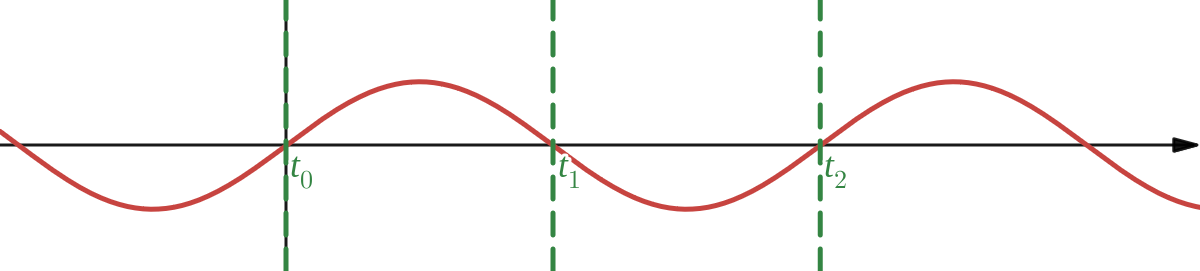
\includegraphics[scale=0.3]{../figures/period_times.png}
\end{center}

\begin{itemize}
	\item Il primo range sarà dato da $t_0 = 0$ a $t_1$, inteso come il punto dove $V_s$ interseca per la prima volta l'asse delle ascisse. Questo sarà quindi il range dove $V_s$ è \textit{positiva};
	\item Il primo range sarà dato da $t_1$ (calcolato prima) a $t_2$, inteso come il punto dove $V_s$ interseca per la seconda volta l'asse delle ascisse (cioè $V_s$ completa un ciclo). Questo sarà quindi il range dove $V_s$ è \textit{negativa};
\end{itemize}

Lo studio del comportamento del circuito per tutti gli altri range temporali sarà quindi derivabile dalla periodicità di $V_s$ (le due situazioni che studieremo si ripeteranno ciclicamente nel tempo).

Vediamo quindi il comportamento del circuito in entrambe le situazioni, preso $D$ come diodo \textit{ideale}:
\begin{itemize}
\item $t_0 < t < t_1$ \\
In questo caso risulterà che $D$ è posto fra un potenziale positivo all'anodo e il ground al catodo. Segue che molto probabilmente sarà in conduzione, e in tal caso $V_u$ vedrà il voltaggio $V_s$:
$$
V_u = V_s = V_m \sin(\omega t)
$$

\par\smallskip
\textbf{\textsf{Verifica}}

Abbiamo posto $D$ in conduzione, quindi imponiamo corrente positiva:
$$
I_D  = \frac{V_s}{R_L} > 0
$$
per cui l'ipotesi è verificata.

\item $t_1 < t < t_2$ \\
In questo caso notiamo che $D$ si trova in polarizzazione negativa, per cui probabilmente sarà in interdizione. In tal caso sul lato destro del circuito non passera nessuna corrente, e $V_u$ sarà nulla:
$$
V_u = 0 \, \mathrm{v}
$$

\par\smallskip
\textbf{\textsf{Verifica}}

Abbiamo posto $D$ in interdizione, quindi imponiamo tensione sotto la soglia di interdizione:
$$
V_D = -5 \, \mathrm{V} < V_\gamma \approx 0.7 \, \mathrm{V}
$$
per cui l'ipotesi è verificata.

\end{itemize}

Abbiamo quindi ottenuto che il circuito rettificatore, almeno nel caso ideale, equivale ad un \textit{cortocircuito} per tensioni positive, e ad un \textit{circuito aperto} per tensioni negative. Il risultato è che la forma d'onda del generatore $V_s$ viene rettificata:
\begin{center}
	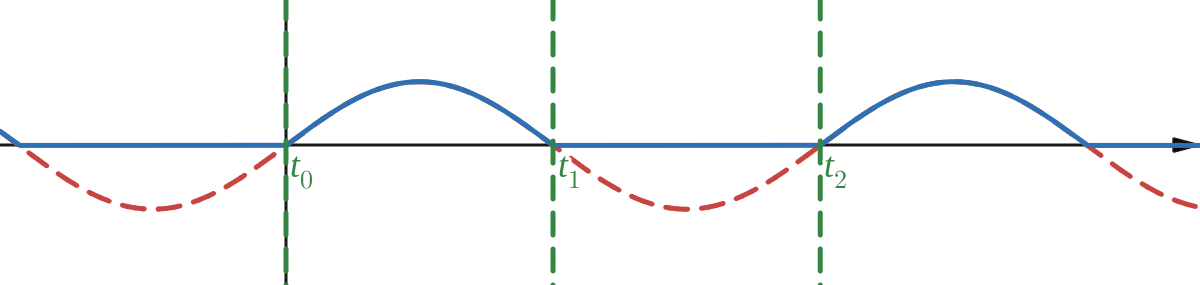
\includegraphics[scale=0.3]{../figures/rect_ideal.png}
\end{center}

\subsubsection{Circuito rettificatore a caduta costante}
Vediamo adesso cosa accade se studiamo il circuito rettificatore sfruttando un modello più accurato del diodo di quello ideale, cioè il modello a \textit{caduta costante}. In tal caso notiamo 2 differenze principali:
\begin{enumerate}
\item Innanzitutto, quando entra in conduzione, il diodo presenterà una caduta di potenziale $V_\gamma$ (che modellizziamo con un generatore di tensione):

\begin{center}
\begin{circuitikz}
	\draw (0,2) to[american voltage source, l=$V_s$] (0, 0);
	\node[ground] at(0,0) {};
	\draw (0,2) to[battery2, l=$V_\gamma$] (4,2) to[resistor, l=$R_L$] (4,0);
	\node[ground] at(4,0) {};
	\draw (4,2) -- (5, 2);
	\node[anchor=west] at(5,2) {$V_u$};
\end{circuitikz}
\end{center}

Notiamo che prendiamo $V_\gamma$ come:
$$
V_\gamma \approx 0.7 \, \mathrm{V}
$$
secondo quanto detto finora.
Questo significherà che il voltaggio in uscita $V_u$, preso $D$ in conduzione, non sarà più equivalente a $V_s$, ma avremo da considerare la caduta:
$$
V_u = V_s - V_\gamma, \quad I_D = \frac{V_s - V_\gamma}{R}
$$
e la corrente cambia di conseguenza.

\item La seconda differenza diventa chiara nel momento in cui proviamo a svolgere la verifica del caso in conduzione. Dovrà infatti essere che:
$$
I_D = \frac{V_s - V_\gamma}{R} > 0 \implies V_s > V_\gamma
$$
cioeè l'ipotesi di conduzione vale soltanto nel caso in cui $V_s$ riesce a superare la soglia $V_\gamma$. Questo significa che avremo due fenomeni sulla forma d'onda di $V_u$:
\begin{enumerate}
	\item Un \textit{ritardo di conduzione} sul fronte dell'onda che parte da $0 \, \mathrm{V}$;
	\item Un \textit{anticipo di spegnimento} sul fronte dell'onda che va a ricadere su $0 \, \mathrm{V}$.
\end{enumerate}

Ritardo di conduzione ed anticipo di spegnimento sono identici ed uguali a $\Delta t$. Calcoliamo tale intervallo notando che vogliamo risolvere:
$$
V_s = V_\gamma = V_m \sin(\omega t), \quad \sin(\omega t) = \frac{V_\gamma}{V_M}, \quad \omega t = \sin^{-1} \left( \frac{V_\gamma}{V_m} \right) 
$$

$$
\implies \Delta t = \frac{1}{\omega} \sin^{-1} \left( \frac{V_\gamma}{V_m} \right) 
$$

\end{enumerate}

Visualizziamo quindi su un grafico il risultato dell'adozione del diodo a caduta costante come modello nel rettificatore. 

\begin{center}
	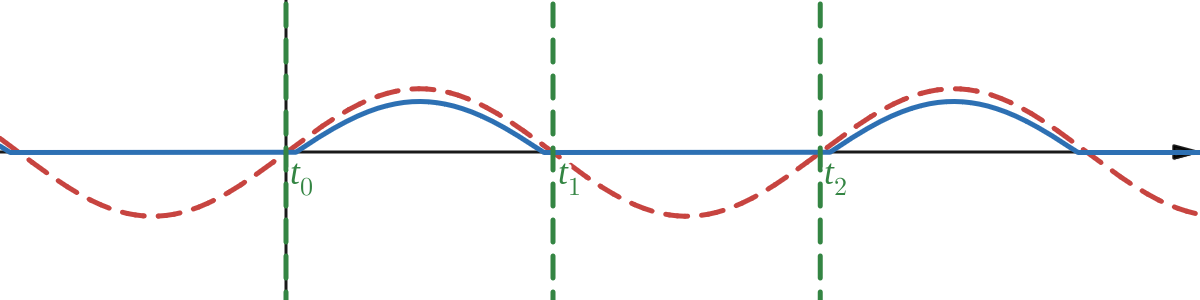
\includegraphics[scale=0.3]{../figures/rect_nonideal.png}
\end{center}

Abbiamo che i picchi del segnale dopo il rettificatore sono stati ridotti (appunto dalla caduta costante), e abbiamo dei ritardi e degli anticipi della regione in cui il segnale viene troncato al di sopra di $0 \, \mathrm{V}$ (in sostanza passiamo più tempo vicino agli $0 \, \mathrm{V})$. 

\end{document}
